%%%%%%齋藤研究室レジュメテンプレート%%%%%%% 2024

\documentclass[a4j]{jsarticle}
\usepackage[utf8]{inputenc}
\usepackage{amsmath,amssymb,amscd,amsthm}
\usepackage{ascmac,fancybox} 
\usepackage{bm}
\usepackage{mathtools}
\usepackage{multicol}
\usepackage{graphicx}
\usepackage[dvipdfmx]{color}
\usepackage{algorithm}%擬似コードを書く場合
\usepackage{algorithmic}%擬似コードを書く場合
\usepackage{tcolorbox}
\usepackage{marginnote}
%%%% ↓algotithmic の \REQUIRE と \ENSURE の表記を変更する
\renewcommand{\algorithmicrequire}{\textbf{Input:}}
\renewcommand{\algorithmicensure}{\textbf{Output:}}
%%%% ↑algotithmic の \REQUIRE と \ENSURE の表記を変更する
\def \QED{\hfill $\Box$}%証明終了の記号

% 新しいカウンターを定義
\newcounter{sectioncounter}[section] % セクションごとにリセット
\renewcommand{\thesectioncounter}{\thesection.\arabic{sectioncounter}} % 形式を1.1, 1.2に設定

% コマンドの定義
\newcommand{\itextgt}[2][]{%
    \refstepcounter{sectioncounter}% カウンターを進める
    \textgt{#2~\thesectioncounter}% 定義番号付きで出力
    \ifx#1\empty\else\label{#1}\fi% ラベルを設定(オプション)
}

%%%%%%%本文%%%%%%% 
\title{第8回\\学部3年後期ゼミナール発表資料}
\author{青山和樹}
\date{2024年12月9日}

\begin{document}

\maketitle

%%目的%%
\section*{発表の目的}
テキスト\cite{text}の
\begin{itemize}
	\item 5.1 Examples of codes
	\item 5.2 Kraft inequality
\end{itemize}
について発表する.


%%目次%%
\tableofcontents

\clearpage

%%本文%%

エントロピーの定義に対して, 情報の圧縮に関する基本的な限界という意味を与える. 圧縮は, データソースに対して, 頻繁に出現するものに短い説明を与え, 出現頻度の低いものに長い説明を割り当てることによって達成される. ここでは, 「瞬時符号(instantaneous code)」という概念を定義し, その後クラフトの不等式(Kraft inequality)を証明する.

\section{Example of codes}

\begin{itembox}[l]{\itextgt{定義}(情報源符号(codeword))}
	確率変数$X$に対する情報源符号$C$とは$\mathcal{X}$($X$の値域)から$\mathcal{D}^*$($D$元アルファベットからなる有限長の文字列の集合)への写像である. $C(x)$を$x$に対応する符号語とし, $l(x)$を$C(x)$の長さとする.
	\begin{align}
		C : \mathcal{X} \rightarrow \mathcal{D}^*
	\end{align}
\end{itembox}\\

\itextgt{例}\quad $\mathcal{X}=\{\text{red}, \text{blue}\}$, アルファベット$\mathcal{D}=\{0, 1\}$に対して
\begin{itemize}
	\item $C(\text{red}) = 00$
	\item $C(\text{blue}) = 11$
\end{itemize}
となるような情報源符号が考えられる.\\

\begin{itembox}[l]{\itextgt{定義}(平均符号語長(expected length))}
	平均符号語長$L(C)$は確率関数$p(x)$に対する確率変数$X$の情報源符号$C$によって
	\begin{align}
		L(C) & = \sum_{x \in \mathcal{X}} p(x)l(x) \\
		     & = \mathbb{E}[l(X)]
	\end{align}
	で表される.
\end{itembox}\\

\itextgt{注意}\quad 一般性と失うことなく, $D$元アルファベットを$\mathcal{D} = \{0, 1, \ldots, D-1\}$と仮定できる\\

\itextgt[example-1]{例}\quad 確率変数$X$を次の分布と符号語の割り当てを持つとする.
\begin{equation}
	\begin{split}
		&\mathbb{P}[X = 1] = \frac{1}{2}, \quad \text{符号語} C(1) = 0,\\
		&\mathbb{P}[X = 2] = \frac{1}{4}, \quad \text{符号語} C(2) = 10,\\
		&\mathbb{P}[X = 3] = \frac{1}{8}, \quad \text{符号語} C(3) = 110,\\
		&\mathbb{P}[X = 4] = \frac{1}{8}, \quad \text{符号語} C(4) = 111,\\
	\end{split}
\end{equation}\\
\begin{align}
	H(X) & = -\frac{1}{2}\log \frac{1}{2} -\frac{1}{4}\log \frac{1}{4}-\frac{1}{8}\log \frac{1}{8}-\frac{1}{8}\log \frac{1}{8} \\
	     & = 1.75 \quad \text{bits}                                                                                            \\[1em]
	L(C) & = \mathbb{E}[l(X)]                                                                                                  \\
	     & = \frac{1}{2}1 + \frac{1}{4}2 + \frac{1}{8}3 + \frac{1}{8}3                                                         \\
	     & = 1.75  \quad \text{bits}
\end{align}\\
$X$のエントロピー$H(X)$は1.75ビットであり, この情報源符号の平均符号語長$L(C)$も1.75ビットである. よって今回の場合では, エントロピーと平均符号語長が一致する情報源符号が得られた. またこの符号では, 任意のビット列を$X$のシンボル列に一意に復号できる. 例えば, ビット列0110111100110はシンボル列134213に復号される.\\

\itextgt{例}\quad 別の簡単な例として, 確率変数$X$を次の分布と符号語の割り当てを持つとする.
\begin{equation}
	\begin{split}
		&\mathbb{P}[X = 1] = \frac{1}{3}, \quad \text{符号語} C(1) = 0,\\
		&\mathbb{P}[X = 2] = \frac{1}{3}, \quad \text{符号語} C(2) = 10,\\
		&\mathbb{P}[X = 3] = \frac{1}{3}, \quad \text{符号語} C(3) = 11,\\
	\end{split}
\end{equation}\\
例\ref{example-1}と同様に, この符号も一意に復号可能である. しかしこの場合, エントロピーは$l\log 3 \approx 1.58$ビットであり, 平均符号語長は1.66ビットである. よって$\mathbb{E}[l(X)] > H(X)$となる.\\

\itextgt{例}\quad モールス符号\\
モールス符号は, 英字アルファベットを表現するために4種類の記号トン, ツー, 文字間スペース, 単語間スペースからなる, 比較的効率的な情報源符号である. 頻繁に使用される文字(例:E)は短い符号列(トン)で表され, 頻度の低い文字(例:Q)は長い符号列(ツーツートンツー)で表される. しかし, この符号は4種類の記号でのアルファベットの最適な表現ではない. 実際, 多くの可能な符号語が使用されていない. その理由は, 文字の符号語に空白が含まれず, 各符号語の末尾にのみ文字間の空白が存在するためである. また, 空白の後に別の空白が続くことがない. この制約の下で構築できる符号列の数を計算することは興味深い問題である. この問題はシャノンによって1948年の元の論文で解かれた.\\

これから, 符号に対するより厳密な条件を段階的に定義していく. そこで$x^n$を$(x_1, x_2, \ldots, x_n)$と表す.\\

\begin{itembox}[l]{\itextgt{定義}(非特異(nonsingular))}
	情報源符号$C$が非特異とは, $X$の値域のすべての要素が$\mathcal{D}^*$の異なる文字列に対応するときである.
	\begin{align}
		x \neq x^\prime \Rightarrow C(x) \neq C(x^\prime)
	\end{align}
\end{itembox}\\

\itextgt{解説}\quad つまり情報源符号$C$が単射であるとき\\

\itextgt{例}\quad 非特異符号\\
$\mathcal{X} = \{A, B, C\}$として, $C(A) = 0,\quad C(B) = 10,\quad C(C) = 11$\\

\itextgt{例}\quad 特異符号\\
$\mathcal{X} = \{A, B, C\}$として, $C(A) = 0,\quad C(B) = 0,\quad C(C) = 10$\\

\itextgt{解説}\quad 非特異は$X$の単一の値を曖昧なく記述するには十分である. しかし通常は, $X$の値の列を送信する場合が多い. このような場合は, 任意の2つの符号語の間に特別な記号(カンマなど)を追加することで, 復号可能性を保証できる. ただし, これは特別な記号の非効率的な使用となる. より効率的な方法として, 自己終端(self-punctuaring)または瞬時符号(instantaneous)のアイデアを発展させることができる. シンボル$X$の列を扱うことから, 符号を拡張する.\\

\begin{itembox}[l]{\itextgt{定義}(符号$C$の拡張(extension))}
	情報源符号$C$の拡張$C^*$は$\mathcal{X}$の有限系列から$\mathcal{D}^*$への写像であり,
	\begin{align}
		C(x_1x_2\cdots x_n) = C(x_1)C(x_2)\cdots C(x_n)
	\end{align}
	で表される.\\
	ここで, $C(x_1)C(x_2)\cdots C(x_n)$は対応する符号語の連接(concatenation)を示す.
	\begin{align}
		C^* : \mathcal{X}^* \rightarrow \mathcal{D}^*
	\end{align}
\end{itembox}\\

\itextgt{例}\quad $C(x_1) = 00, \quad C(x_2) = 11$であれば, $C(x_1x_2) = 0011$\\

\begin{itembox}[l]{\itextgt{定義}(一意復号可能(uniquely decodable))}
	一意復号可能であるとは, その情報源符号の拡張$C^*$が非特異であるときである.
\end{itembox}\\

\itextgt{解説}\quad 一意復号可能な符号では, 符号化された任意の文字列に対して, それを生成する情報源系列は1つしか存在しない. しかし, 元の文字列の最初のシンボルを特定するためにも, 文字列全体を確認しなければならない場合がある.\\

\itextgt{例}\quad $\mathcal{X} = \{A, B, C\}$として, $C(A) = 0,\quad C(B) = 01,\quad C(C) = 011$とする. このとき001011は$ABC$に復号される.\\

\begin{itembox}[l]{\itextgt{定義}(語頭符号(prefix code)・瞬時符号(instantaneous code))}
	符号が語頭符号または瞬時符号であるとは, どの符号語も他の符号語の語頭(先頭部分)にならないことである.
\end{itembox}\\

\itextgt{解説}\quad 瞬時符号は符号語の終わりが即座に認識できるため, 先の符号語を読まずに復号できる. 瞬時符号は自己終端符号でもある. 例えば例\ref{example-1}の符号によって生成された2進数文字列01011111010は0, 10, 111, 110, 10として解釈される.\\

これらの定義の入れ子構造は図\ref{class-of-codes-figure}に示される. 様々な種類の符号の違いを説明するために, $x \in \mathcal{X}$に対する符号語$C(x)$の割り当て例を表\ref{class-of-codes-table}に示す.\\

\begin{figure}[H]
	\centering
	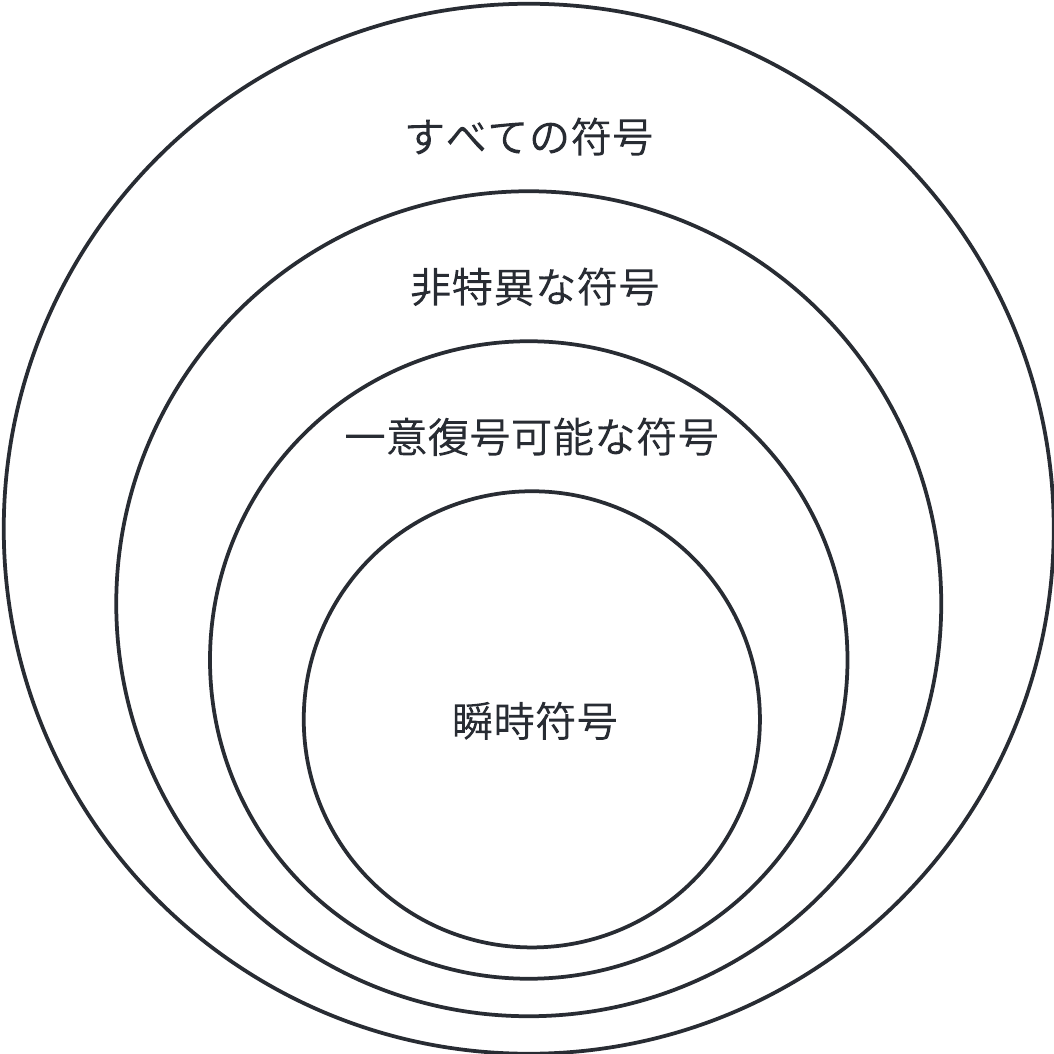
\includegraphics[width = 5.0cm]{class_of_codes.png}
	\caption{符号のクラス}
	\label{class-of-codes-figure}
\end{figure}

\begin{table}[h]
	\centering
	\caption{符号のクラス}
	\begin{tabular}{ccccc}\hline
		$X$ & 非特異 & \begin{tabular}{c}
			               非特異であるが \\一意復号可能ではない
		               \end{tabular} & \begin{tabular}{c}
			                               一意復号可能であるが \\瞬時符号でない
		                               \end{tabular} & 瞬時符号                                \\\hline
		1   & 0      & 0                                     & 10                                    & 0   \\
		2   & 0      & 010                                   & 00                                    & 10  \\
		3   & 0      & 01                                    & 11                                    & 110 \\
		4   & 0      & 10                                    & 110                                   & 111 \\\hline
	\end{tabular}
	\label{class-of-codes-table}
\end{table}

\section{Kraft inequality}

%%参考文献%%
%\newpage
\begin{thebibliography}{99}
	\bibitem{text}T.M.Cover and J.A.Thomas, Elements of Information Theory, Second Edition, John Wiley \& Sons, 2006.
\end{thebibliography}

\end{document}